\chapter{Referencial Teórico}
\section{Software Analytics}
Durante muito tempo, a falta de dados em projetos de software foi uma constante.
Agora com o auxílio da internet e dos projetos de software livre, existem tantos
dados relacionados a projetos de software que é manualmente impossível de analisá-los
por completo\cite{artAndScience}. Ao fim de 2012, pesquisas mostraram que o \textit{Mozilla Firefox} 
teve 800.000 bug reports e outras plataformas como \textit{Sourcefoge.net}
e o \textit{Github} hospedam 324.000 e 11.2 milhões de projetos, respectivamente\cite{informationNeeds}.

Para ser capaz de manipular essa grande quantidade de dados, muitos pesquisadores
se voltaram para o uso e \textit{analytics}, ou seja, o uso de análises, dados e
raciocínio sistemático para tomar decisões. Podemos definir \textit{Software Analytics}
como: `A análise de dados de software para gerentes e engenheiros de software, 
com o objetivo de capacitar individuos e times de desenvolvimento, a ganhar e difundir 
conhecimento a partir de seus dados para tomar melhores decisões'\cite{informationNeeds}.

Hoje é comum empresas como Google, Facebook e Microsoft aplicarem métodos de data
science diariamente em seus projetos. Além disto, o número de conferencias neste
tópico aumentou bastante, sendo as duas mais importantes \textit{Mining Software
Repositories} (MSR) e a \textit{PROMISE Conference on Repeatable Experimentes in Software
Engineering}, cada uma com um foco diferente, sendo a MSR procupada com a coleta dos dados
enquanto a PROMISE com a eficacia e repetibilidade da análise de dados.

As metodologias ágies, acompanhando o crescimento da utilização do Data Science no
mercado, também vem utlizando desta tecnica para otimizar a evolução de produto. Um
dos meios de aplicar a análise de dados em um ciclo ágil é utlizar uma abordagem 
analitica de planejamento de release, ou seja utilizar fontes externas e internas
de dados para planejar as entregas futuras do produto de software. 

A análise de dados obtidos de ferramentas de versionamento de código, como o Git,
Bazaar, Subversion ou CVS podem trazer informações importantes a respeito da evolução
de um projeto de software, do nível de engajamento dos desenvolvedores, número de defeitos
e do desenvolvimento distribuido e muitos outros tópicos\cite{artAndScience}. O Github,
uma das ferramentas mais utilizadas de versionamento de código, fornece uma api que permite
a extração de dois tipos de dados:

\begin{itemize}
\item \textbf{Metadados:} Os metadados fornecidos são informações associadas a cada
commit ou issue, são elas: criador(a), data, mensagem do commit ou issue, a branch e repositório,
e o escopo do commit ou issue. Além disto, na mensagem do commit podem haver referencias a outros
desenvolvedores, bugs ou outros commits e issues.
\item \textbf{Snapshots:} O código fonte do projeto, que pode ser obtido em diferentes
fases do desenvolvimento, já que a ferramente permite que um usuário avance ou retroceda
dentro dos commits. Desta forma, é possivel analisar o código de um projeto referente
a vários periodos diferentes.
\end{itemize}

Abaixo na\ref{github_api} podemos ver o digrama de classes da API fornecida pelo
Github, com base nesta imagem, é possivel ver que as issues e informações dos commiters
são exportadas a partir de um ponto comum de acesso.

\begin{figure}[h]
    \centering
    \label{github_api}
        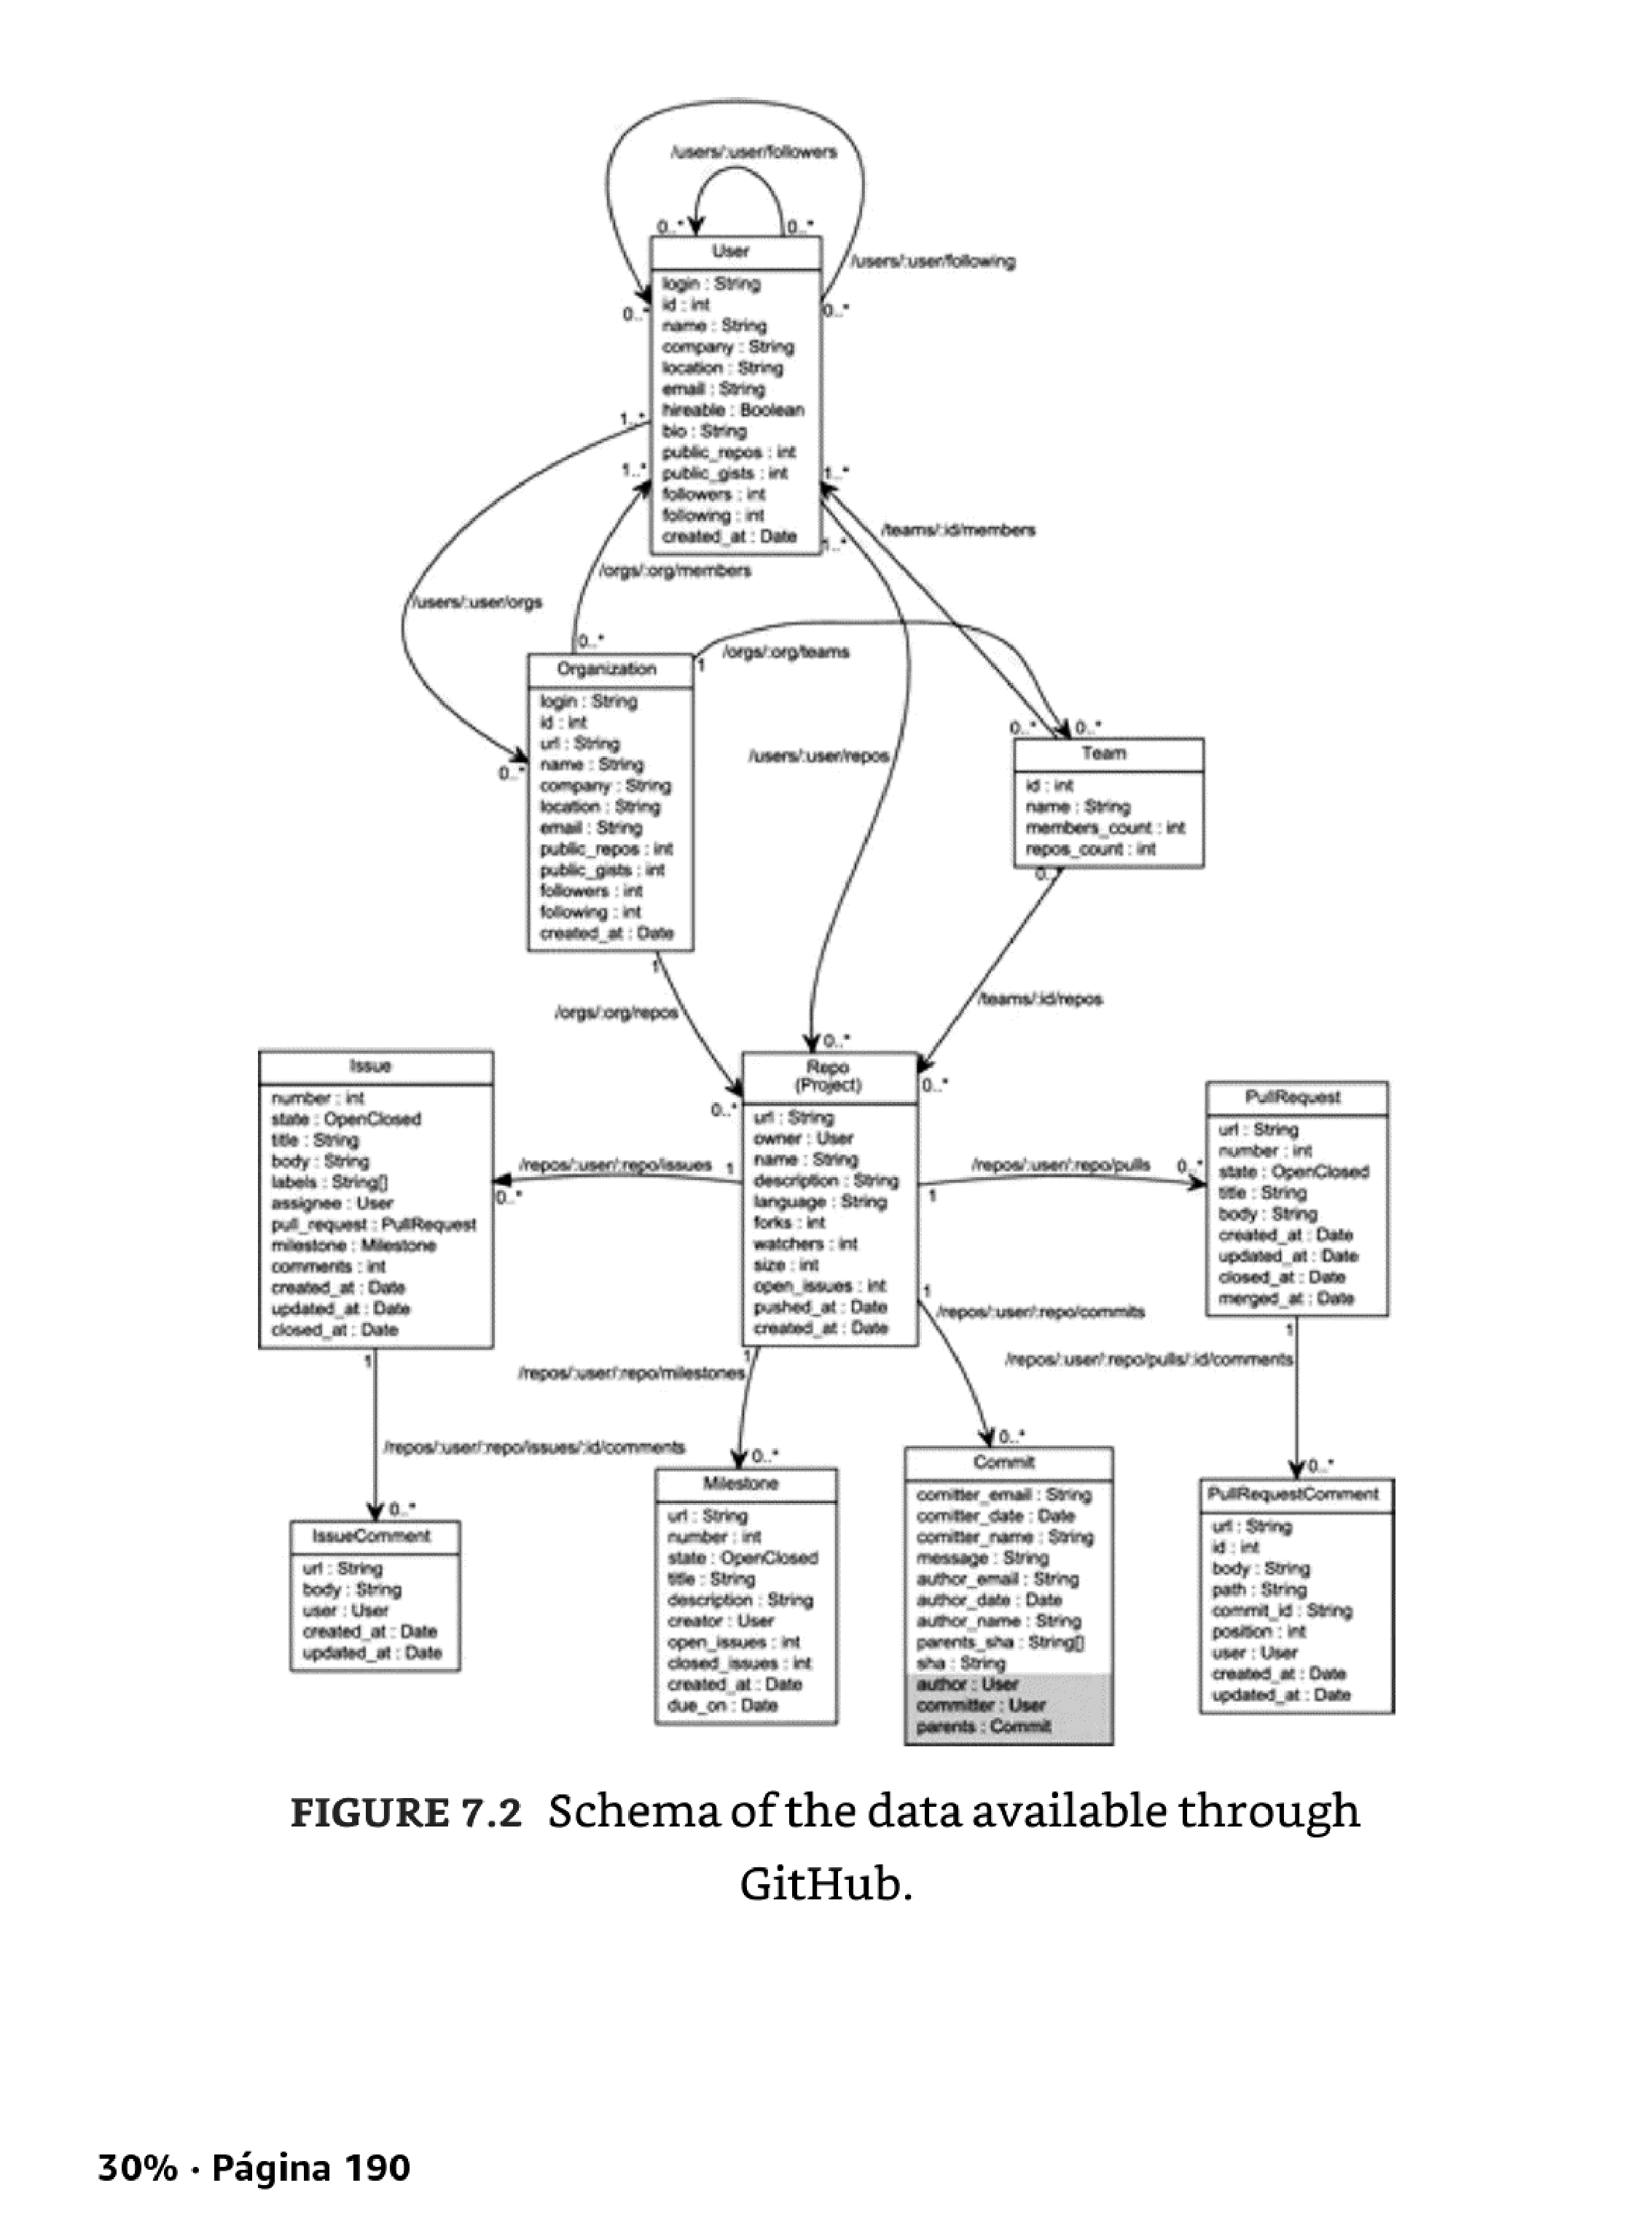
\includegraphics[keepaspectratio=true,scale=0.3]{figuras/github_api_diagram.eps}
    \caption{Representação UML da API do Github}
\end{figure}

Utilizando-se das informações mostradas na\ref{github_api} é possivel utlizar
\textit{Software Analytics} para possibilitar uma melhor tomada de decisão em um
repositório que utilize da ferramenta Github para organizar o trabalho.

\section{Centralidade de Redes}

Centralidade é um conceito fundamental e um dos tópicos mais estudados na análise 
de redes sociais, ele determina o grau de importancia de um vértice dentre todos
os outros dentro de uma rede. O conceito de centralidade de redes já foi aplicado a diversos contextos,
dentre eles: investigar a influencia de redes interorganizacionais, estudos de relevância,
vantagens em redes de troca, competencia em organizações formais, oportunidades de emprego 
e diversos outros campos do mercado e ciência\cite{centrality}.

\subsection{Page Ranking}
